\section{Overvejelser (og Redskaber)}

\begin{frame}
\frametitle{Snorken}
	\begin{quote}
	Snorken er en åndedrætsforstyrrelse, hvor drøbelen eller den bløde gane sættes i vibrationer af en blokering i luftvejene.
	Snorken er en særdeles udbredt søvnforstyrrelse.
	\end{quote}	

	\begin{itemize}
		\item Kan være stærkt signal på søvn
		\item Også tegn på dårlig søvn
		\item Hvordan ved man hvem der snorker?
	\end{itemize}
\end{frame}

\section{Proof of concept}

\begin{frame}
\frametitle{Proof of concept}
Vi betragter stilstandsperioder som indikator på søvn.

\only<1>{
\begin{figure}
	\begin{minipage}{\linewidth}
		\begin{subfigure}{0.5\linewidth}
			\centering
			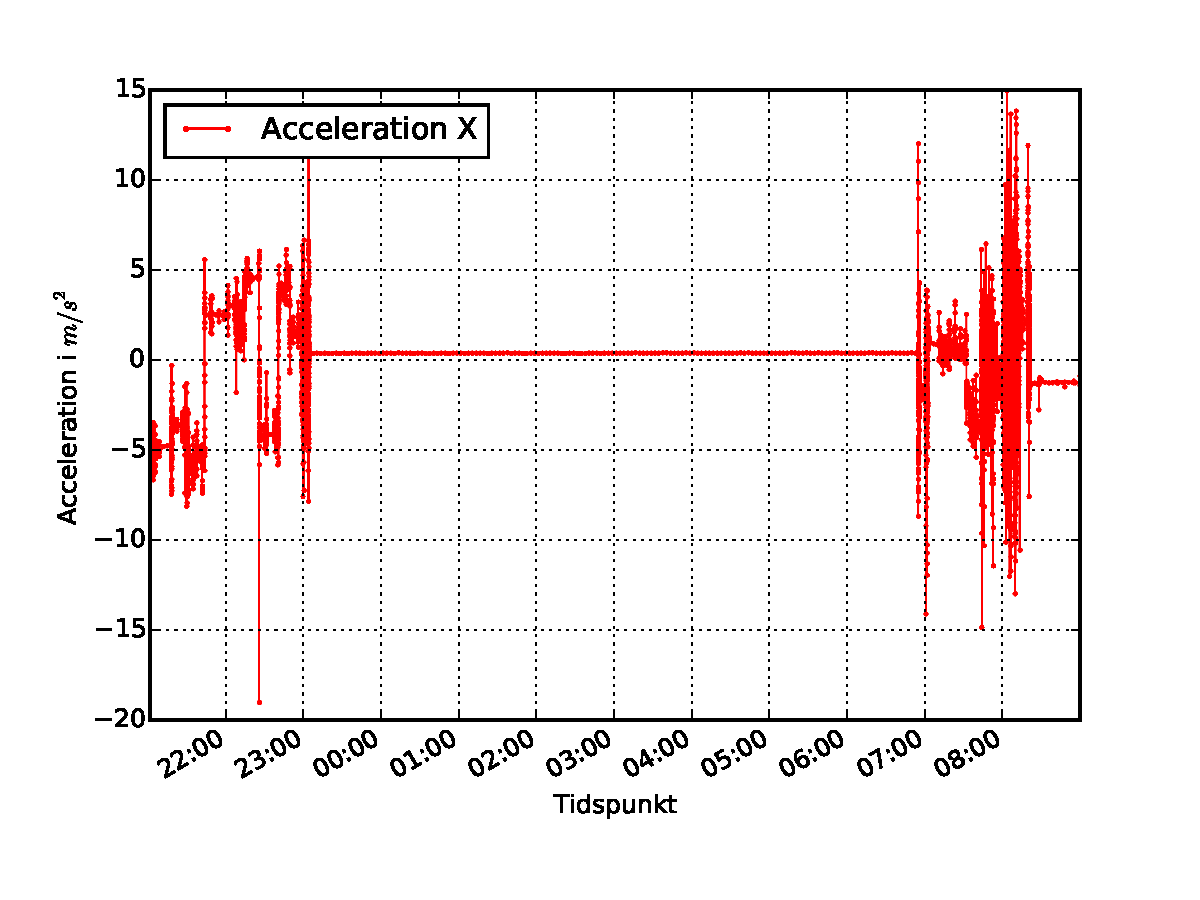
\includegraphics[scale=0.27, trim = 1cm 1cm 1cm 1cm, clip]{../Report/grafik/kombi_figur/acceleration-plot}
			\caption{Rå accelerations-data.}\label{fig:rawaccplot}
		\end{subfigure}
		\begin{subfigure}{0.5\linewidth}
			\centering
			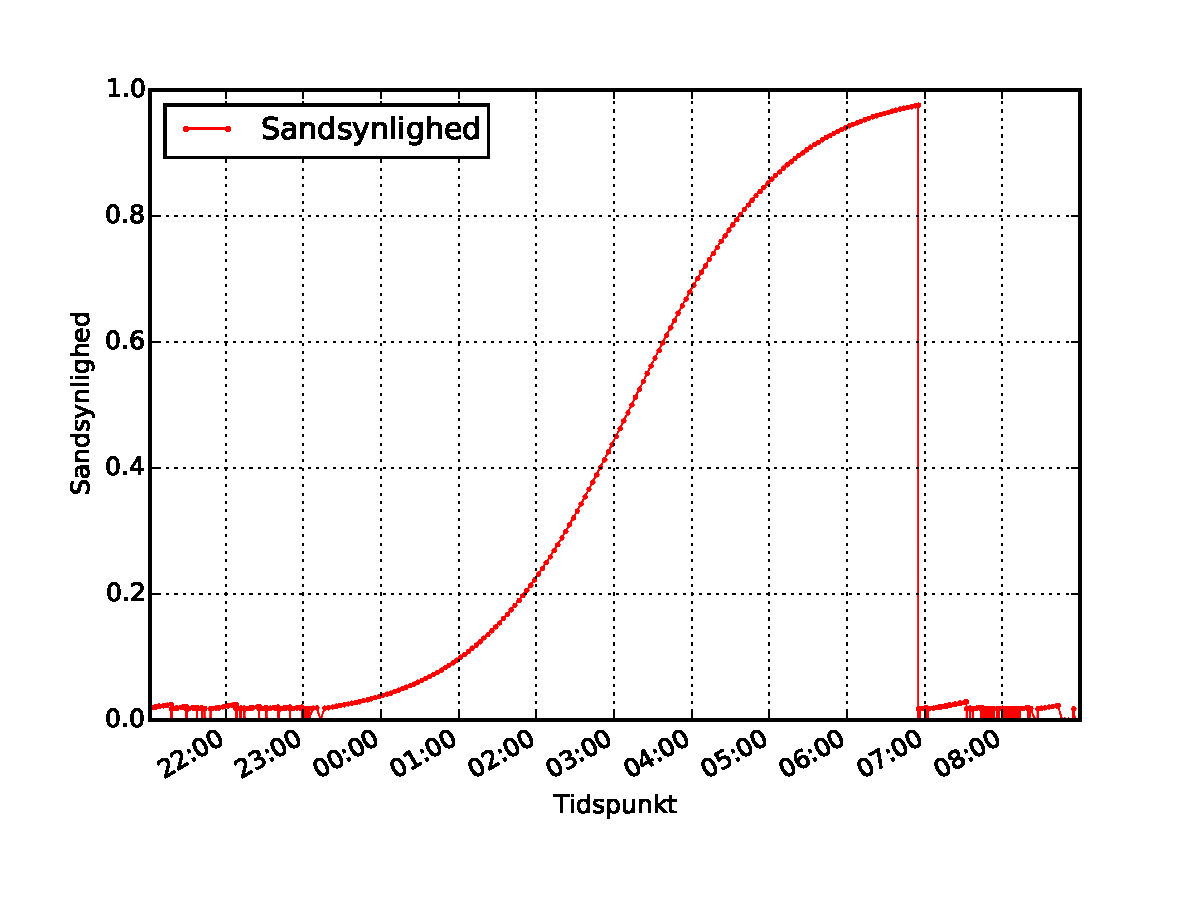
\includegraphics[scale=0.27, trim = 1cm 1cm 1cm 1cm, clip]{../Report/grafik/kombi_figur/acceleration-sleep-estimate-plot}
			\caption{Accelerations-søvnestimering.}\label{fig:sleepcalcaccplot}
		\end{subfigure}
	\end{minipage}\\[1ex]%
\end{figure}
}

\only<2>{
\begin{figure}
	\begin{minipage}{\linewidth}
		\begin{subfigure}{0.32\linewidth}
			\centering
			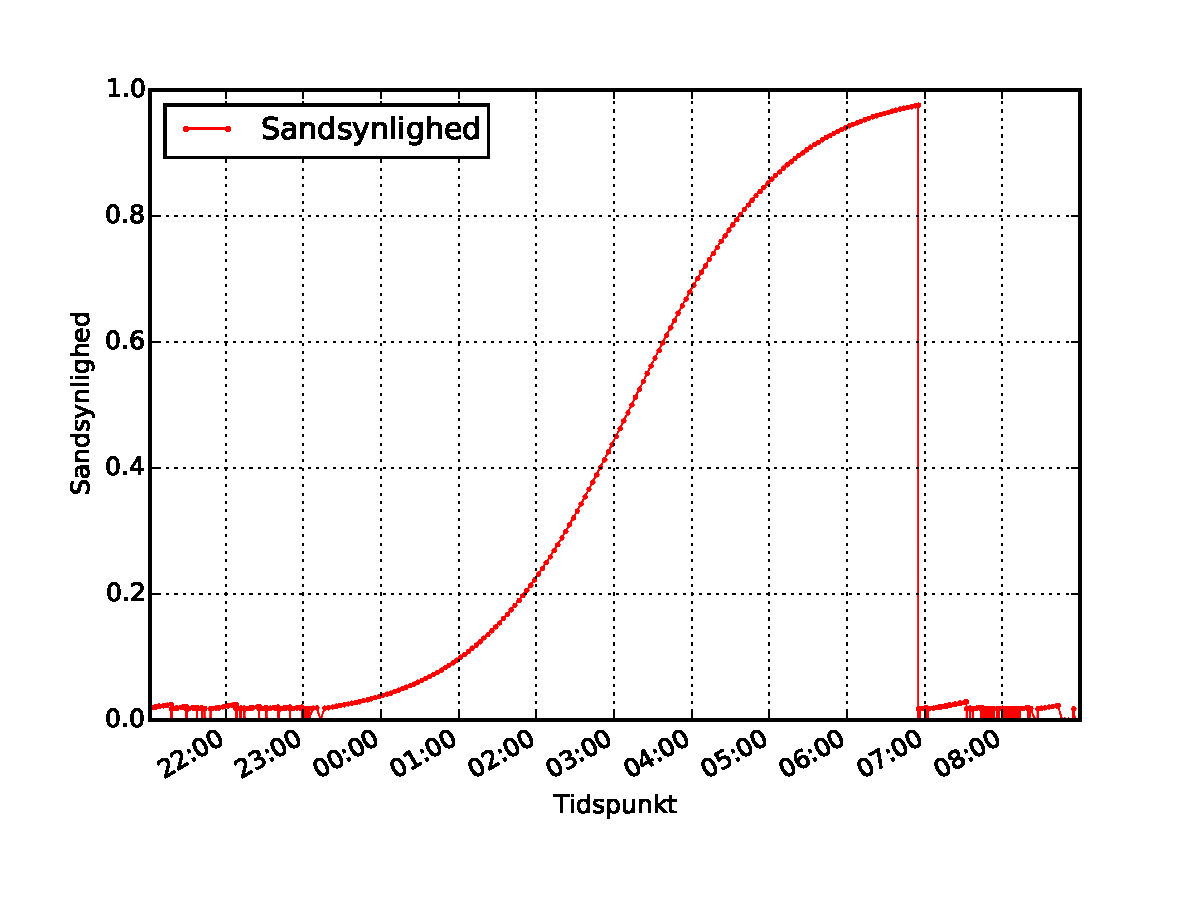
\includegraphics[scale=0.2, trim = 1cm 1cm 1cm 1cm, clip]{../Report/grafik/kombi_figur/acceleration-sleep-estimate-plot}
			\caption{Accelerations-søvnestimering.}\label{fig:sleepcalcaccplot}
		\end{subfigure}
		\begin{subfigure}{0.32\linewidth}
			\centering
			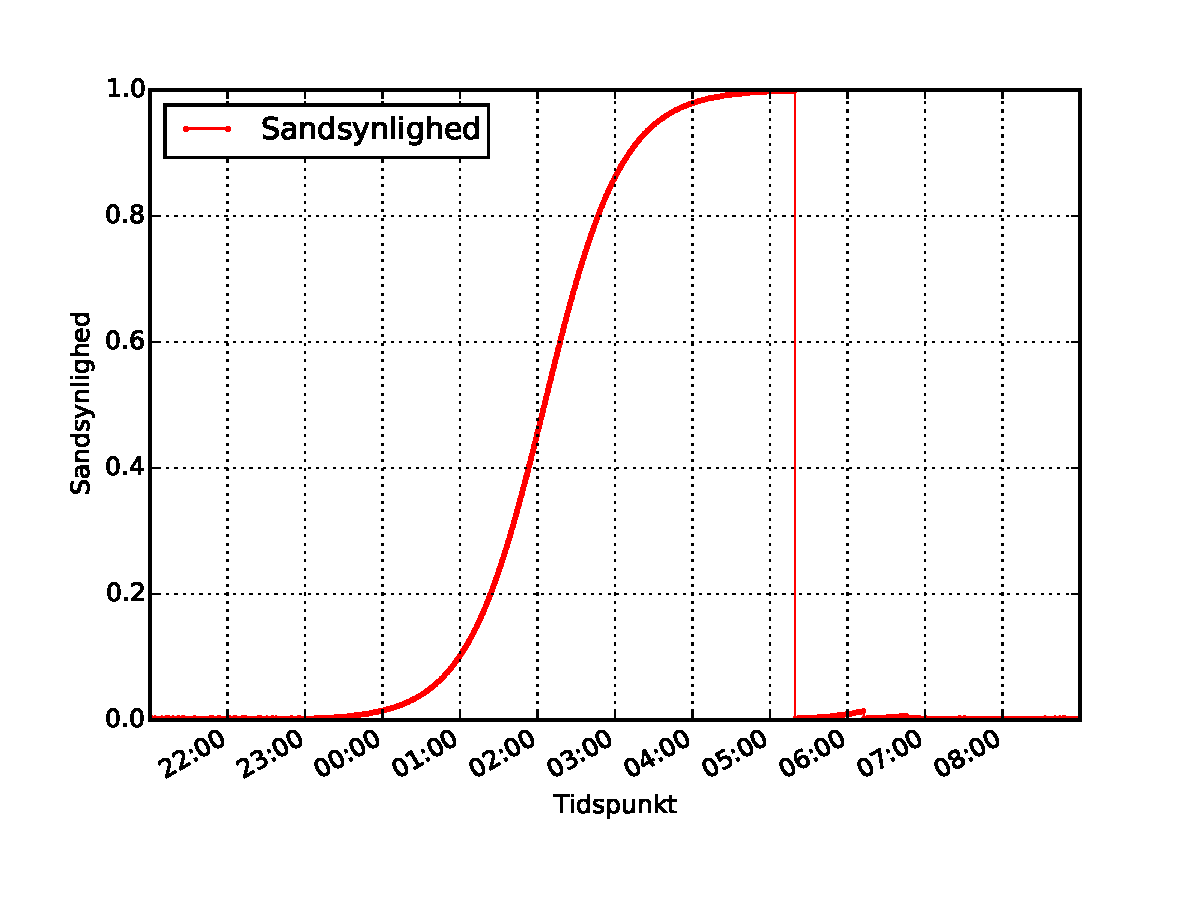
\includegraphics[scale=0.2, trim = 0cm 1cm 1cm 1cm, clip]{../Report/grafik/kombi_figur/amplitude-sleep-estimate-plot}
			\caption{Amplitude-søvnestimering}\label{fig:sleepcalcamplplot}
		\end{subfigure}
		\begin{subfigure}{0.32\linewidth}
			\centering
			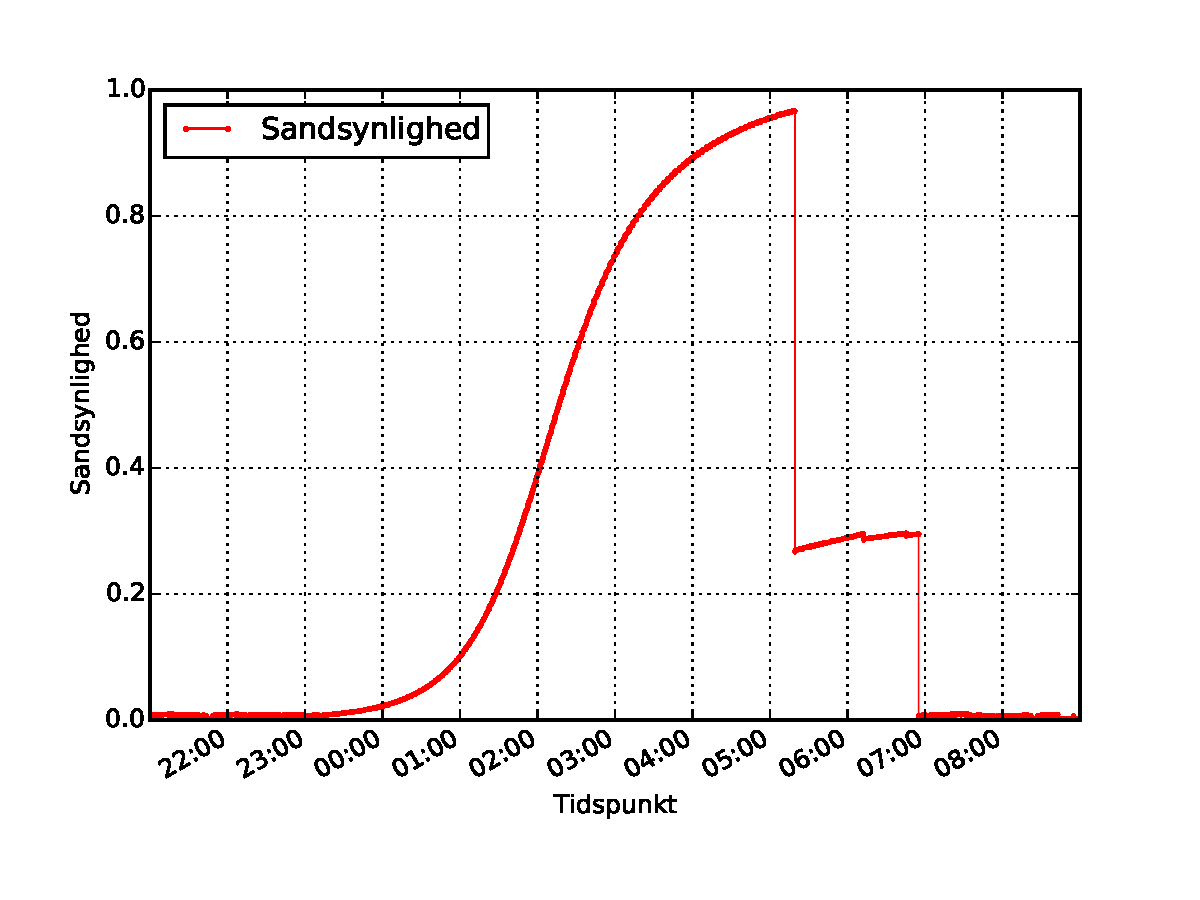
\includegraphics[scale=0.2, trim = 1cm 1cm 1cm 1cm, clip]{../Report/grafik/kombi_figur/combined-sleep-estimate-plot}
			\caption{Kombineret søvnestimering}\label{fig:sleepcalcombine}
		\end{subfigure}
	\end{minipage}\\[1ex]%
\end{figure}
}

\only<3>{
\begin{figure}
	\begin{minipage}{\linewidth}
		\begin{minipage}{\linewidth}
		
		\begin{subfigure}{\linewidth}
			\centering
			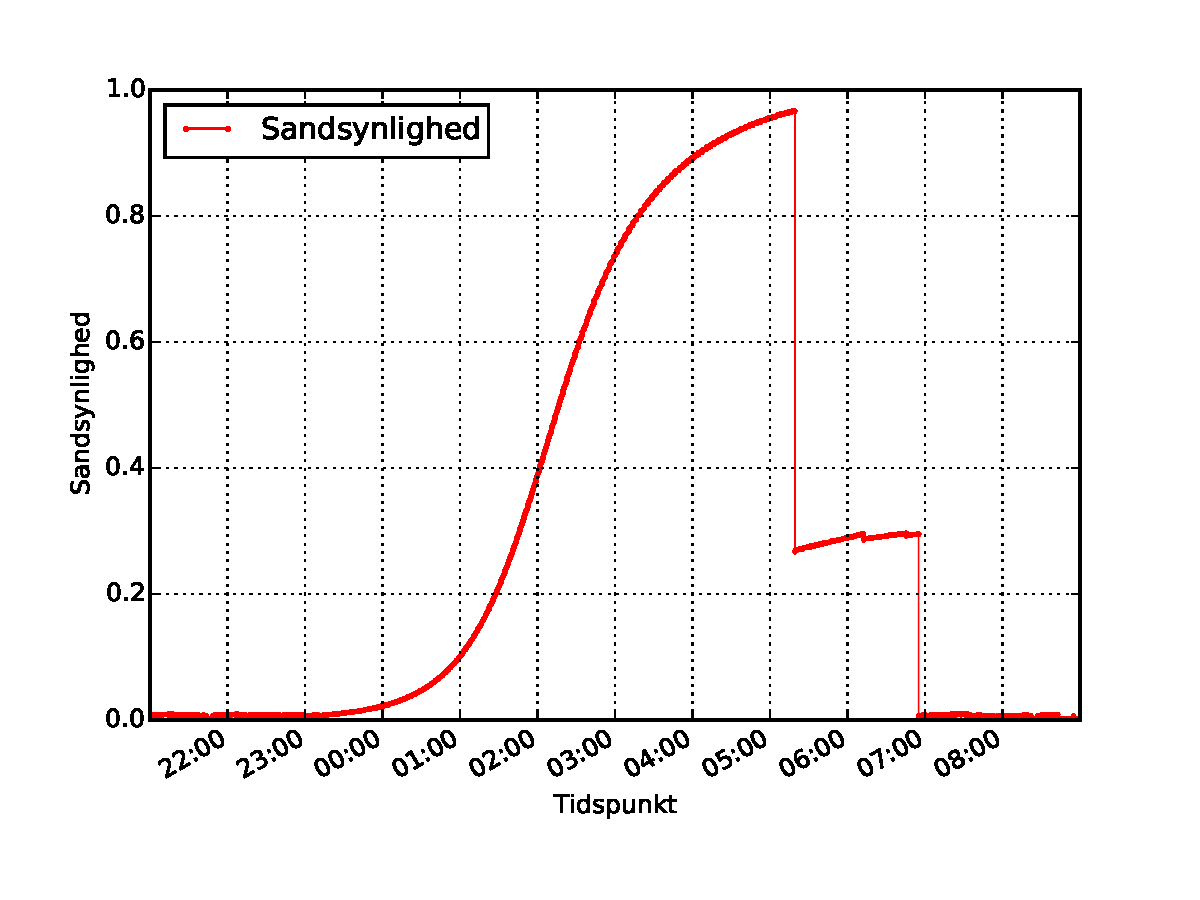
\includegraphics[scale=0.2, trim = 1cm 1cm 1cm 1cm, clip]{../Report/grafik/kombi_figur/combined-sleep-estimate-plot}
			\caption{Kombineret søvnestimering}\label{fig:sleepcalcombine}
		\end{subfigure}
		\end{minipage}
		\begin{minipage}{\linewidth}
		\begin{subfigure}{\linewidth}
			\centering
			\begin{tabular}{|c|c|c|}
			\hline starttid & sluttid & sandsynlighed \\ 
			\hline 2015-04-21 23:11 & 2015-04-22 05:19 & 0.97 \\ 
			\hline 2015-04-22 05:19 & 2015-04-22 06.45 & 0.29 \\ 
			\hline 
			\end{tabular}
			\caption{Samlet søvnaggregeringsresultat.}\label{fig:finalagg}
		\end{subfigure}
		\end{minipage}
	\end{minipage}\\[1ex]%
\end{figure}
}
\end{frame}

\section{Demonstration}
\begin{frame}
	\frametitle{Demonstration}
	Med telefon eller skærmbilleder???? - her en huskeliste
	\begin{itemize}
		\item Husk at vis indstillingsmenuen
		\item Vis forsiden
		\item Hvad info er relevant - søvngraferne bør nok udelades
	\end{itemize}
\end{frame}


\section{Refleksion og konklusion}
\begin{frame}
\frametitle{Refleksion og konklusion}
\begin{itemize}
	\item Kan vi benytte produktet udenfor psykiatrien?
	\item Vi har ikke begrænset os - mulighed for videreudvikling åben
	\begin{itemize}
		\item Bør arbejdes videre på
		\item Inddrage andre faktorer såsom snorken og fysisk aktivitet
	\end{itemize}
	\item Stammer vores data fra patienten eller en anden i husstanden?
	\begin{itemize}
		\item Centralt at vi måler præcist og på den rigtige hvis søvnestimering skal indgå i behandlingen
	\end{itemize}
	\item \textbf{Ændring i adfærd}
\end{itemize}
\end{frame}

